\section{Economic model}\label{sect:constraints}


This section illustrates how to constraint the protocol parameters to achieve the desired TL scheme behavior.

\paragraph*{Preamble}
As previously mentioned, \shortname assumes all the participants to be rational agents. 
This means they are driven by economic interests and they will always try to maximize their profit. 
So, there is no interest in \secret itself, but only in its economic value.
%
Also, as \shortname is built upon secret sharing, it is pivotal to analyze the scenario by referencing to the behavior of groups of adversaries, and not of single users.
Thus, we reference by \coalition a generic malicious coalition of users that team up to break the TL ahead of disclosure time.

\paragraph*{Method}
To limit the attack surface, we model \shortname as a negative sum game to all the possible adversarial coalitions. 
In other words, we impose that anyone who tries to break the TL schema has to face costs greater than the maximum achievable revenues. 
To ensure this condition, we develop a set of constraints among the economic parameters.
% so that any rational agent that takes part to the protocol will comply with its rules.
However, to define each of them we need to identify the maximum revenue an attacker can achieve.
For this purpose, we focus on the best possible attack scenario, or rather the one in which an adversarial coalition ideally completes its entire strategy without interference by other parties.

Before going into details, we fix the first trivial constraint.
It simply captures, in a single expresion, the relation among the amounts discussed in the previous section:

\begin{equation}\label{eqbase}
\Wshare < \BH < \RH < \Wsecret
\end{equation}

In the following we address how coalitions could try to attack the protocol based on the role of its members and the time at which the attack could be performed.
For the sake of clarity, Subsections~\ref{sect:mal_sha} and ~\ref{sect:mal_own} do not take into account the \texttt{\algowhistleblowshare} function, which will be discussed in as special case in Subsection~\ref{sect:impact_wh}.
Finally, Section~\ref{sect:economic_po} addresses how to constraint \PO.


%In the description we gave so far only the basic protocol operating scheme was presented, but no mention was made about the ratio between the economic constraints that have to be imposed on the parameters.
% The protocol is in fact vulnerable because it is exposed to coalitions of attackers that can be both {\em internal} and {\em external} to the TL mechanism.
%However, since the economic (dis-)incentives are the only way to achieve the compliance of rules, it is required to identify the targets which these rules are addressed to, so that the desired outcome is obtained. In particular, the target of the described protocol is strictly time dependent, as the participants have to protect the secrecy of \secret before the disclosure time, and as after \td they have to make sure it to be disclosed.

\begin{algorithm}[t]
	\caption{SC function to disclose the share after \td}\label{algo:disclose}
	\begin{algorithmic}[1]
		\MyAlgBlock{input}
		\Desc{$sc$}{\hspace*{1.5em}smart contract identifier}
		\Desc{$i$}{\hspace*{1.5em}index of the submitted share}
		\Desc{$\share_i$}{\hspace*{1.5em}the $i$-th share}
		\vspace{0.6em}
		\Procedure{Disclose}{$sc, i, \share_{i}$}
		\If{$sc.\state = \statelocked$ \textbf{and} $sc.\states[i] = \statepaid$}
		\If{$\primtime \geq sc.\td$ \textbf{and} $\primtime < sc.\te$}
		\If {$\primhash{\share_i} = sc.\Cshare{}[i]$}
		\State $sc.\shares \left[ i \right] \gets \share_{i}$
		\State $sc.\numdisclosed\ += 1$
		\State $sc.\states[i]\gets \statedisclosed$
		\State $p_1 \gets sc.\numdisclosed \ge sc.\K$
		\State $p_2 \gets \primtime > \te$
		\State $p \gets p_1 \wedge p_2$
		\State $\primwithdraw{sc}{caller}{\RH}{p}$
		\EndIf
		\EndIf
		\EndIf
		\EndProcedure
	\end{algorithmic}
\end{algorithm}

\subsection{Protection against malicious shareholders}\label{sect:mal_sha}

Being the shareholder rational agents, they will consider if is worth to try breaking the TL before \td or not.
To perform a successful attack, a shareholder has to team up with other $\K - 1$ ones in order to reconstruct \secret, sell it to a buyer, and finally whistleblow it.
In that event, \coalition would earn at most by selling and by whistleblowing,\footnote{The coalition \coalition could setup an additional external contract between \coalition and the buyer to be sure to gain both \V and \Wsecret.} leading the protocol to failure. 
The alternative, i.e. do not break the TL and submit the $k$ shares after \td, would lead to a gain equal to the sum of the rewards. 
To avoid the first scenario we can impose:
%
%\begin{equation}\label{eqbalance1}
%\tag{$1^*$}
$\K \cdot \RH  > \V + \Wsecret$.
%\end{equation}

Yet, in order to to earn $\K \cdot \RH$, the coalition \coalition should wait until \td, whereas $\V + \Wsecret$ could be collected earlier.
For this reason, in \shortname we use a stricter formulation of the constraint, obtained by comparing the revenue earned by whistleblowing and the total amount of bids already paid \coalition to get the shares:

\begin{equation}\label{eqcoscom2}
\K \cdot \BH > \V + \Wsecret
\end{equation}

Constraint (\ref{eqcoscom2}) addresses secrecy (time $t < \td$), however, when the disclosure time passes, the objective of the TL turns into facilitating the disclosure.
In this setting, threshold cryptography may obstacle the release of \secret, offering additional opportunities to malicious shareholders and coalitions of them.
In fact, $\N - \K + 1$ shareholders could wait for $\K - 1$ others to submit their share and then lead the TL instance to a stall by refusing to submit their ones and wait for a buyer willing to pay \V to gain access to the secret.
To avoid this issue, we introduce the constraint:  

\begin{equation}\label{eqcoscom4}
(\N - \K + 1) \cdot \RH  > \V
\end{equation}

Here the contribution of the term $\Wsecret$ disappears as the role of whistleblower is no longer admissible after \td. The inequality holds because the shareholders are authorized to collect their rewards \RH only in case the TL results in a successful outcome\footnote{An alternative approach to reduce stalls without the need of a termination time and deferred rewards would be to grant an extra reward \extrareward to the first \K shareholders that submit the share after \td.
%Timely payment of rewards would encourage this type of attack, as in some situations \coalition could use it to reduce the entry fee while still not publicly disclose the secret (i.e., not write it to the smart contract).
%Such a bonus --- which in total amounts to $\K \cdot \extrareward$ --- would be paid from \PO.
%The latter would contribute positively to inequalities~\ref{eqbalance1} and ~\ref{eqcoscom2}.
%anyhow foreseeing race conditions is not strictly compulsory.
}
(i.e., at least \K shares are submitted before the termination time \te).


\subsection{Protection against malicious owners}\label{sect:mal_own}

All the considerations made about the rationality of the shareholders must also be applied to the owner.
As \owner knows the secret in advance, she could setup fake TL instances for the sole purpose of invoking the \texttt{\algowhistleblowsecret} function and obtain \Wsecret, if this would end up having a positive economic return.
%
%Anyone in possession of the secret can act as a whistleblower, then the owner could be interested in setting up a fake protocol to get $\Wbonus_{\secret}$.
To enforce a negative outcome for this scenario, we need to add the following constraint:

\begin{equation}\label{eqbalance3}
\PO > \Wsecret
\end{equation}

%Since the penalties are enforced by smart contracts, someone might be tempted to prevent the owner from executing the whistleblow protocol, thus replacing~\ref{eqbalance3} by an identity check.  Yet, there is no way to forbid the owner from teaming up with a shareholder, and forming an malicious mixed coalition.  Such a case should be addressed by the addition of:

%\begin{equation}\label{eqbalance7}
%\PO + \BH > \Wbonus_{\secret}
%\end{equation}

%which is a less stringent constraint than~\ref{eqbalance3}.


\subsection{Impact of share whistleblowing function}\label{sect:impact_wh}

The ability to whistleblow shares, which is needed to prevent them to be sold, opens up to more complex strategies that can be performed by coalitions.
A coalition \coalition
% composed by \K shareholders 
could in fact submit some of the controlled shares to the contract before whistleblowing the secret, in order to maximize its revenue.

As the coalition is composed by rational agents, it is possible to determine the optimal number \jopt of shares that \coalition could submit before incurring into penalties or advantaging other participants.
%Indeed, submitting $k$ shares before \td leads to the TL failure, and therefore the impossibility of earning $\Wbonus_{\secret}$, which we remind is greater than $\Wbonus_{\share}$. 
Whistleblowing a share is in fact a public event, observable by anyone, so it could itself trigger other participants' strategies.
%Another aspect we point out is that a share whistleblow is an event observable by all the participants, as the state smart contract is publicly readable. 

The values \N and \K, the number of total shareholders and the threshold, identify two cases to compute  \jopt. \newline \vspace*{-0.5em} \newline
{\em General case.}
In general, a \K-shareholders coalition \coalition is not the only one able to break the TL. 
Each time a share is whistleblown the threshold \K is weakened, and all other $\N-\K$ shareholders and their possible coalitions are triggered as a side effect.
%Let's assume that a first coalition $\coalition ^\prime $ whistleblows a share;
%$\coalition ^\prime $ would earn $\Wshare$, while losing the bid \BH paid to obtain the share.
%
%, accordingly a second coalition $\coalition ^{\prime \prime} $ might form.
%, $\coalition ^{\prime \prime} $ would save \BH in case of an hypothetical \secret reconstruction.
%As $\BH > \Wbonus_{\share}$, then $\coalition ^{\prime \prime} $ would become the most dangerous attacker. \\	%A second coalition $\coalition ^{\prime \prime}$ that only consists of $\K-1$ shareholders would now be able to reconstruct the secret. 
Overall, when $i$ shares have been whistleblown, a quiescent coalition $\coalition^i$ formed by $\K-i$ shareholders, would gain the ability to reconstruct the secret \secret having paid only $(\K-i) \cdot \BH$ to get its shares. 
For this reason, the initial coalition \coalition formed by \K shareholders needs to determine the optimal number of shares \jopt to be whistleblown so that there is no other coalition that can profit from the weakening of \K. In particular, $\coalition$ can determine \jopt by solving the following:	
$$\jopt = \operatorname*{max}_i\ \{i | (\K-i) \cdot \BH > \V + \Wsecret,\ i \in 1,\ldots,\K-1 \}$$
%, while benefit from a cost saving of $i \cdot \BH$ while performing the attack. So, if $i_{inv}$ so that
%$$
%\begin{cases}
%\left( \K - i_{inv} \right) \cdot \BH < \V + \Wbonus_{\secret} \\
%\left( \K - i_{inv} + 1 \right) \cdot \BH > \V + \Wbonus_{\secret} 
%\end{cases}
%$$
If such a \jopt exists, by keeping the assumption of rational agents, the coalition \coalition can submit \jopt shares while still being sure that no other smaller coalition will whistleblow the secret.	\newline \vspace*{-0.5em} \newline
{\em Special case $\K > \lfloor \N/2 \rfloor. $}
In this case, the \K-shareholders coalition \coalition is the only one able to break the TL. 
Specifically, $2\K-\N-1$ shares can be submitted while still preventing the other $\N-\K$ shareholders to reconstruct \secret. 
Please note that such number of submissions could be smaller compared to the one identified by the general case, which is only cost dependent. 
To compute the optimal number of submissions, it is then required to select:
$$ \jopt = \operatorname*{max}\ \{ \left( 2\K - \N - 1 \right) ; \text{ } \jopt _\text{general\textunderscore case} \}$$

Whistleblowing shares permits to gain the extra-revenue $ \Wer = \jopt \cdot \Wshare$.
%
To address it, we formulate a stricter version of Equation~(\ref{eqcoscom2}) by constraining:

\begin{equation}\label{eqcoscom2w}
\K \cdot \BH > \V + \Wsecret + \Wer
\end{equation}


\subsection{Evaluating Costs}\label{sect:economic_po}

Now that we've discussed how to constraint the parameters to prevent misbehavior, we discuss the additional requirements to be satisfied by \PO.
In fact, it is from this amount the owner pays the shareholder profits, or the whistleblower bonuses. 
Overall, the sum of \PO and the shareholder bids $\N \cdot \BH$ must be able to cover the costs for every possible evolution of the TL instance.
The easiest evolution is represented by all the shareholders correctly executing the protocol. To accommodate for this case, we need to impose that the amount stored in the smart contract is enough to pay the shareholder rewards:

\begin{equation}\label{eqpo1}
\PO + \N \cdot \BH \geq \N \cdot \RH
\end{equation}

On the contrary, the TL could fail with $\K-1$ shares whistleblown before the secret itself is whistleblown.
To ensure the smart contract has enough value to be able to pay all the whistleblower bonuses, we impose the following constraint:

\begin{equation}\label{eqpo2}
\PO + \N \cdot \BH \geq (\K-1) \cdot \Wshare + \Wsecret
\end{equation}

As $\BH > \Wshare$, we do not need to discuss mixed evolutions of the TL. In fact, right side of Inequality~(\ref{eqpo2}) reports the worst case amount.
In any other circumstance (i.e., less than $\K-1$ shares whistleblown), 
%disclosure rewards are replaced by whistleblower bonuses, but being $\RH > \Wshare$, 
the Inequality~(\ref{eqpo2}) still holds.

\begin{figure}[t]
	\centering
	\begin{tabular}[b]{| c | c | c | c | c | c |}	
		\hline
		\V & \Wshare & \BH & \RH & \Wsecret & \PO \\
		\hline \hline
		1 & 0.025 &  0.275 &  0.3 &  0.325 &  0.35 \\
   		\hline \hline
		10 & 0.25  &  2.75  &  3   &  3.25  &  3.5  \\
   		\hline \hline
		100 & 0.5   & 25.5   & 26   & 26.5   & 27    \\
		\hline
	\end{tabular}
	\caption{Sample configurations with $\K=5$ and $\N=8$ and $\V \in {1,10,100}$ that respect all the constraints (optimized for minimizing \PO)}
	\label{table:variables}	
\end{figure} 

The constraints (\ref{eqbase}-\ref{eqpo2}) must all hold for any well-formed instance of \shortname. 
They identify the acceptance area for the variables. 
The owner may desire to minimize \PO, while the shareholders would like to maximize the profit $\RH - \BH$.
A more thorough analysis of the ratio among this variables and the different strategies to set them is out of scope in this chapter.
In Table~\ref{table:variables} we show three possible configurations for $\K=5$, $\N=8$, and $\V \in {1, 10, 100}$, which minimize \PO, obtained by constraint programming.
It is worth to remark that in all of the cases we have $\PO < \V$, which is a desirable property.


\subsection{Temp comments}
$\bullet$ What can be learnt from a whistleblowon share?
\newline
$\shareholder_{1}$ submits her share. 
As $\Wbonus_h < \BH$, then there are two options: (i) she is not rational, and (ii) she is rational.
Case (i) is not compatible with our model.
Case (ii) implies that $\shareholder_{1}$ is being playing a strategy.
So, if a shareholder submits a share, then at least one malicious coalition \coalition exists.  
\\
$\bullet$ How much is the cardinality of coalition of Case (ii)?
\newline
Observe that all the shareholders are rational, and \K is the Shamir Secret Sharing threshold.
So, an initial share submission implies that \coalition not only exists, but that it is composed by \K member (i.e., no less than \K shareholders can break the TL, more than that would imply lower profit).
\newline
Please note that the optimal strategy for a \K-members coalition \coalition, is:
$\K \cdot \BH > \V + \Wsecret + \jopt \cdot \Wbonus_h $,
while the best strategy for its competitors is:
$
\left( \K - 1 \right) \cdot \BH > \V + \Wsecret + \left( \jopt - 1 \right) \cdot \Wbonus_h
$.
As $\BH > \Wshare$, \coalition will not consider any strategy involving the submission of more than \jopt shares (i.e., \coalition prevents its adversaries from having a positive return).
Please also note that the strategy of \coalition is addressed by constraint (\ref{eqcoscom2w}) of Section~\ref{sect:constraints}.
\\
$\bullet$ Reduction of disjoint coalitions
\newline
Any strategy jointly performed by $x$ disjoint rational coalitions, $x>1$, is equivalent to the one of a single rational coalition composed by all the shareholders of the $x$ coalitions (i.e., they spent $x \cdot \BH$ to get $x$ shares, and they have to fairly distribute any profit). 
\\
$\bullet$ Overlapping coalitions
\newline
Suppose that a group of shareholders $\mathcal{Z} := \{ \shareholder_1 \cdots \shareholder_{i} \}$ is part of two coalitions, $\coalition^\prime$ and $\coalition^{\prime\prime}$ (i.e., $\mathcal{Z} := \coalition^\prime \cap \coalition^{\prime\prime}$).
For what was said before, one of the two performs the first share submission, so at least one among $\coalition^\prime$ and $\coalition^{\prime\prime}$ has cardinality \K, say $\coalition^\prime$.
The other, $\coalition^{\prime\prime}$ has cardinality less than \K, for obvious reasons.
%
It follows that the action of $\mathcal{Z}$ is successful if $\coalition^{\prime\prime}$ breaks the TL (i.e., it sells and whistleblows \secret) while benefiting from the submission of some shares by $\coalition^\prime$ participants.
If that was the case then the strategy of $\coalition^\prime$ would malformed.
In general it is so when it does not specify ordering, allowed and forbidden shareholders' actions, it does not take into account the global state of TL instance, and when and does not provide for any type of countermeasure for failure to comply with the agreements. 
But this implies that the shareholders in $\coalition^\prime - \{ \shareholder_1 \cdots \shareholder_{i} \}$ are not rational, and this is absurd (i.e., it contradicts rationality assumption).


%\subsection{Variations}\label{sect:variat}

%In this subsection we show how the proposed model can be easily extended to achieve additional goals.

%\subsubsection{Resiliency}
%Until now we always assumed all the parties to be perfect rational agents. However, a number of shareholders \lost might expose their share (i.e., because of negligence, external attacks). In such a case, a coalition of $\K - \lost$ malicious shareholders could reconstruct the secret without the need of sharing the reward with the shareholders that lost their shares.
%To prevent this possibility, the owner could define \lost to be the upper bound of the number of shares that can go misplaced. By integrating this information into equation~(\ref{eqcoscom2}), we are able to nullify the gain for such a coalition:
%\begin{equation}\label{eqcoscom3}
%(\K - \lost) \cdot \BH  > \V + \Wbonus
%\end{equation}




%\paragraph*{Reducing owner pawn}



%pursuing the will to play against the system (i.e., against the shareholders), or could misbehave because of giving up to keep interest into \secret and then trying to get the whistleblower bonus.
%
%To dis-incentivize his misbehavior, we include in our model a reward \RO that the owner will receive in case of successful executions of the protocol.
%

%By defining a relation between \Wbonus and \RO we can impose that even if the owner loses interest in keeping \secret private, he will have a greater benefit from a successful execution of the protocol compared to whistleblowing the secret:

%The introduction of \RO requires to adapt the equality~(\ref{eqbalance}), since this reward has to be paid by the owner:

%\begin{equation}\label{eqbalance4}
%\PO = \N \cdot \profit  + \RO
%\end{equation}

%This way we enforce that the costs for the owner are always greater than the benefits he can obtain from the system (effectively dis-incentivizing his misbehavior). In fact, by combining Equation~(\ref{eqbalance3}) and Equation~(\ref{eqbalance4}), we can derive:

%\begin{equation}\label{eqbalance5}
%\PO > \RO > \Wbonus
%\end{equation}


%\subsubsection{Avoiding owner reward}

%Foreseeing a reward \RO for the owner after \td might be considered as an active role for the owner after \td. This is acceptable in scenarios in which the owner wants to safeguard the publication of the secret \secret at time \td, even though she is expected to return online at a later time to claim her reward.

%As described in Section~\ref{sect:protection}, the owner reward \RO is necessary to prevent gains from an owner who is willing to setup a fake protocol just to claim the whistleblower bonus \Wbonus (at the expenses of the shareholders). 
%An alternative to avoid the owner reward \RO, would be to limit the attack surface of a malicious owner. This can be done by limiting the role of the whistleblower only to the shareholders \shareholder (i.e., the owner can not claim the whistleblower bonus). This is not enough as an attacker could take part to the \shortname protocol with two identities, one in which he plays as the owner, and one in which he plays as a shareholder. To prevent any economic gain from this practice, we can introduce the following additional constraint.

%\begin{equation}\label{noro}
%\PO + \BH > \Wbonus
%\end{equation}

%This way, any coalition of the owner, who knows \secret, and a shareholder, needed to whistleblow, would imply a negative gain.

%\begin{comment}
%UNCOMMENT THIS WHEN FINAL.

%\begin{figure}[tp]
%	\centering
%	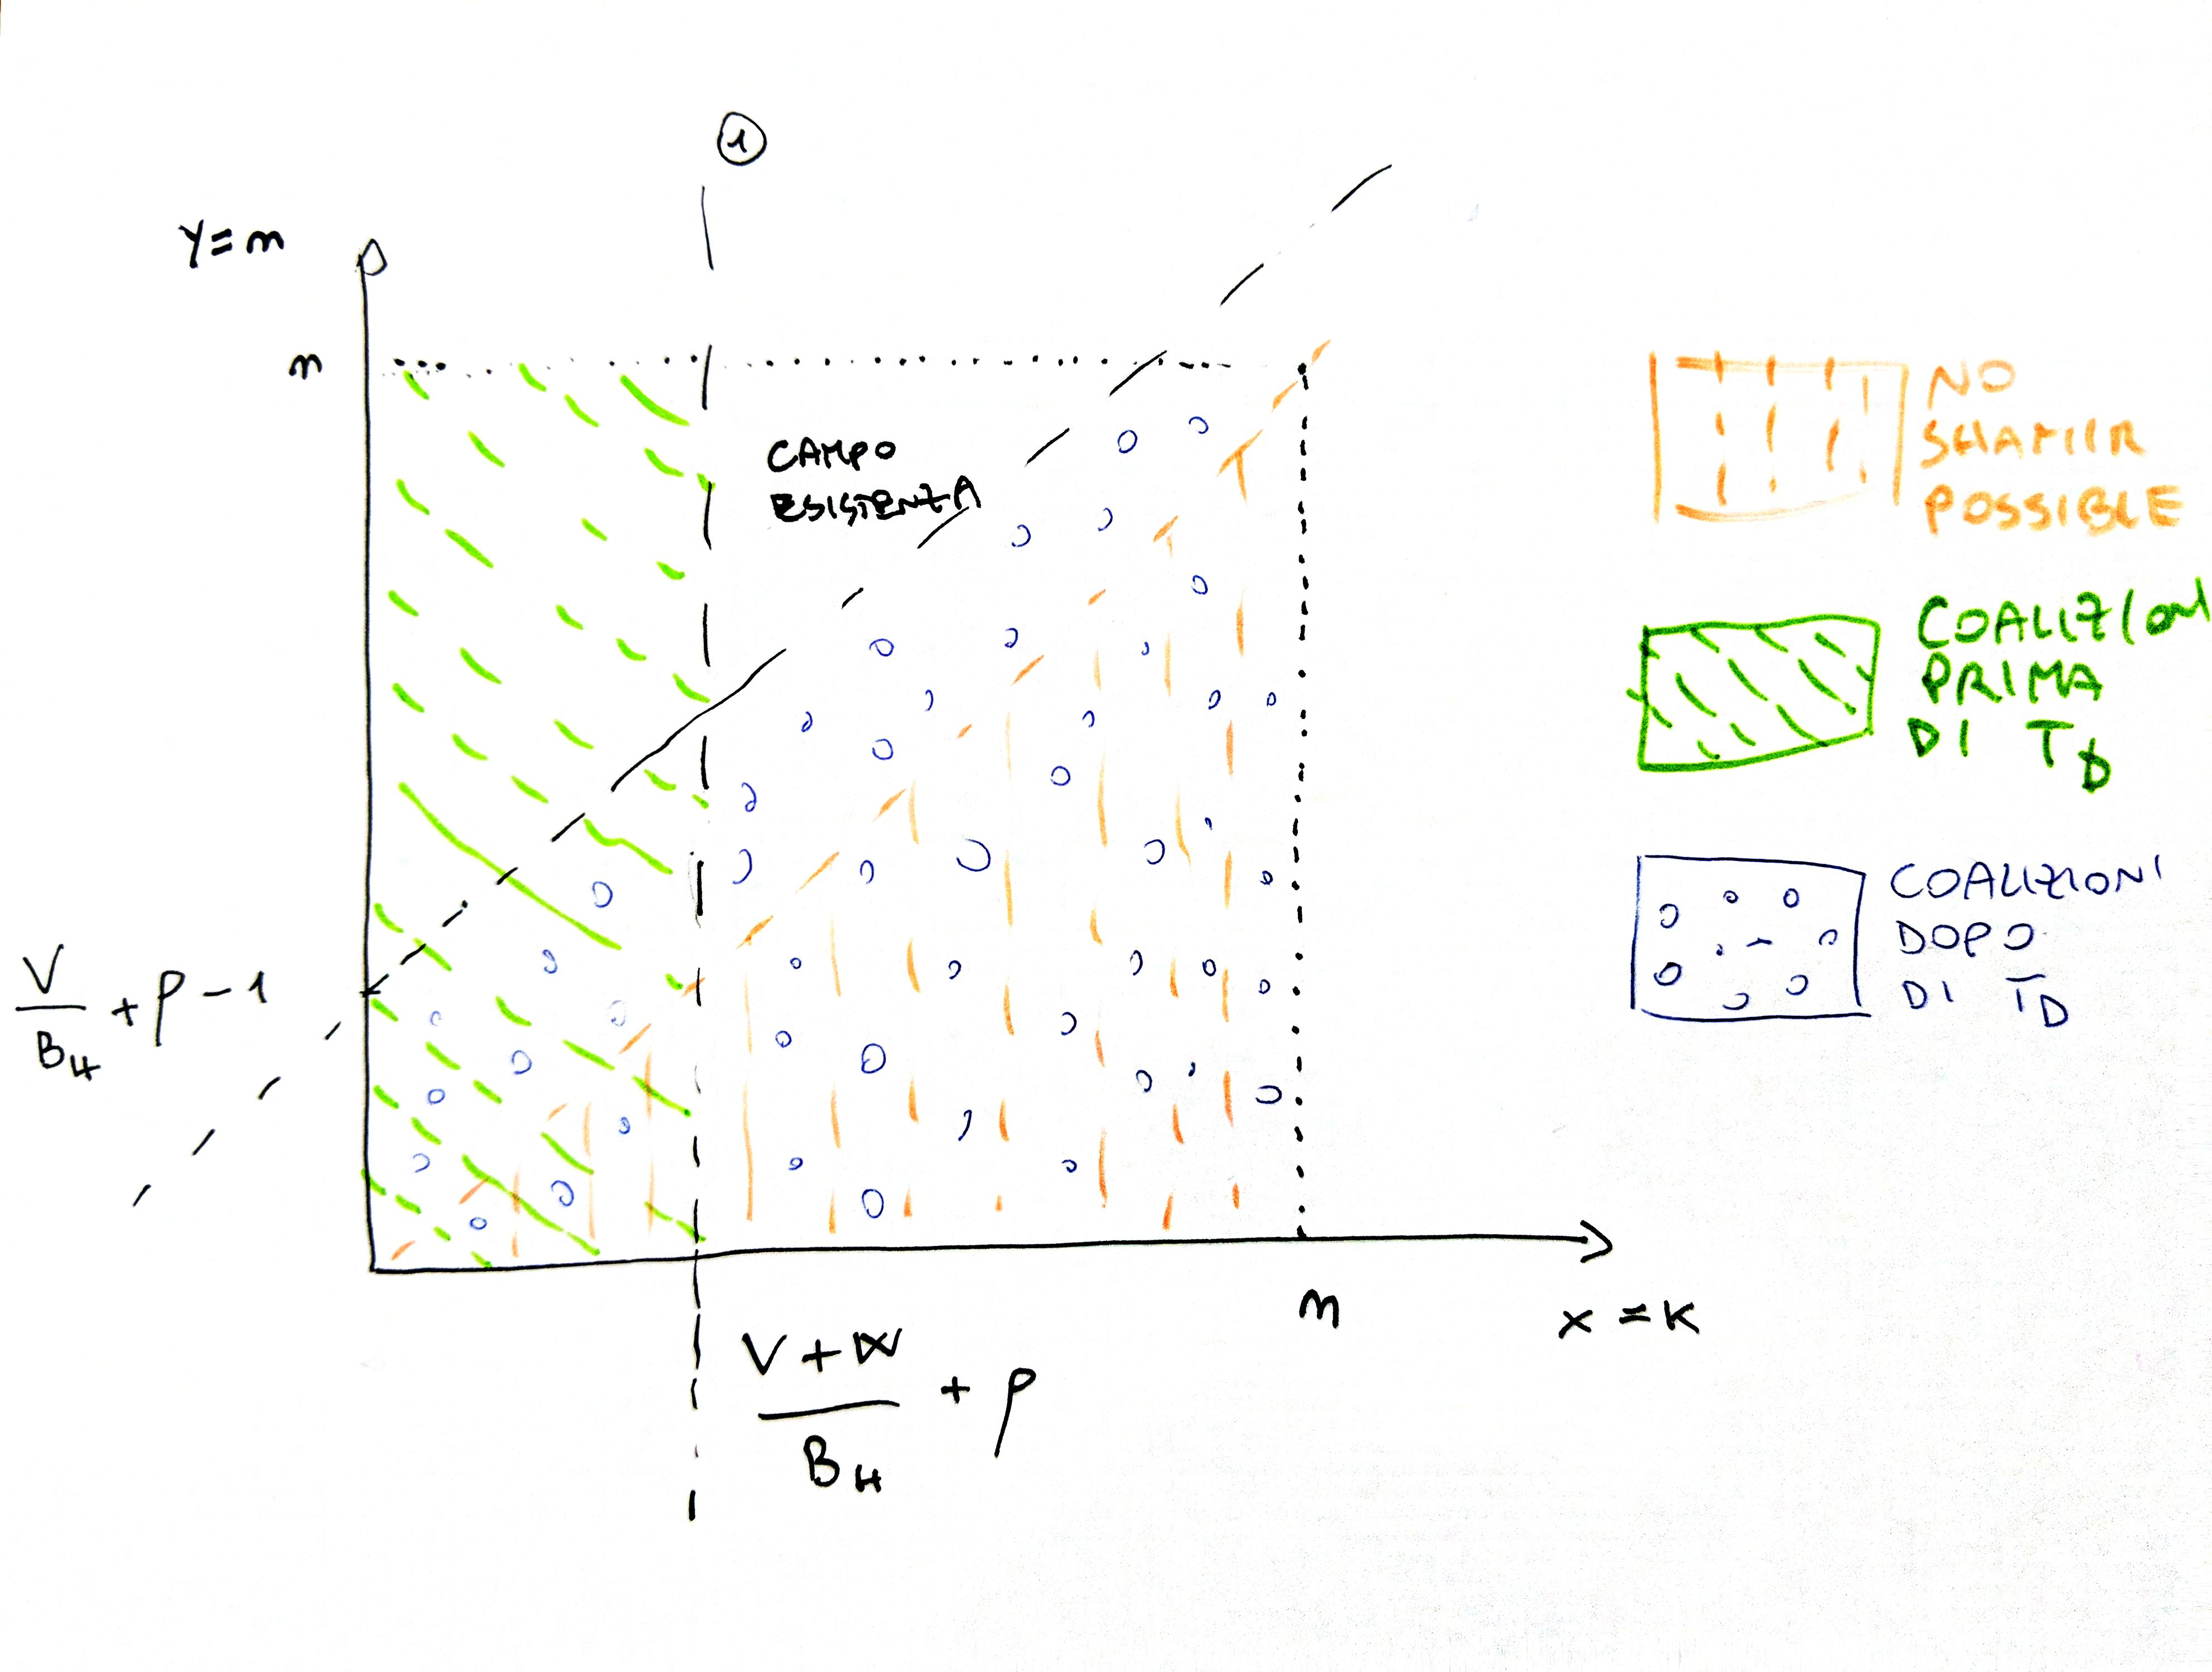
\includegraphics[width=\columnwidth]{fig/constraints}
%	\caption{{\em \shortname} constraints.}
%	\label{fig:constraints}
%\end{figure}
%
%due righe per introdurre la rappresentazione grafica dei vincoli e del campo di esistenza del modello, ATTENZIONE TOGLIERE DALLA FIGURA IL CONTRIBUTO DELLE VARIAZIONI
%\end{comment}